% -*- TeX:Soft -*-
% JMarkov User's Guide by Riano and Goez

\documentclass[11pt,letterpaper]{article}
\usepackage{amsmath}
\usepackage{graphicx}
\usepackage[USenglish]{babel}
\usepackage{algorithm}
\usepackage{algorithmic}
\usepackage{listings}
\usepackage{cite}
%\usepackage{flafter}
\usepackage{xspace}
\usepackage[T1]{fontenc}
\usepackage[latin5]{inputenc}

%\usepackage{amsfonts}
%\usepackage{optprog}
\usepackage{color}
\usepackage{makeidx}
%\usepackage{flafter}% Causes floats to show AFTER cited
\usepackage{epstopdf}
\usepackage{xspace}
\usepackage[breaklinks]{hyperref}



\definecolor{darkgreen}{rgb}{0.00,0.50,0.25}

\title{jMarkov User's Guide}
\author{  Germ\'an Ria\~no and Julio G�ez  \\
Universidad de Los Andes}
\date{}

\newcommand {\cA}{\ensuremath \mathcal{A}}
%\newcommand {\cS}{\ensuremath \mathcal{S}}
\newcommand {\lil}{\lstinline}
\DeclareMathOperator*{\argmax}{argmax}
\newtheorem{rem}{Remark}
\newcommand{\HB}{\mathbf{H}^{\bullet}}
\newcommand{\LB}{\mathbf{L}^{\bullet}}
\newcommand{\UB}{\mathbf{U}^{\bullet}}
\newcommand{\Gb}{\mathbf{G}_{\bullet}}
\newcommand{\Ub}{\mathbf{U}_{\bullet}}
\newcommand{\bP}{{\mathbf P}}
\newcommand{\bM}{{\mathbf M}}
\newcommand{\ba}{{\mathbf a}}
\newcommand{\be}{{\mathbf e}}
\newcommand{\bA}{{\mathbf A}}
\newcommand{\bB}{{\mathbf B}}
\newcommand{\bF}{{\mathbf F}}
\newcommand{\bG}{{\mathbf G}}
\newcommand{\bg}{{\mathbf g}}
\newcommand{\bQ}{{\mathbf Q}}
\newcommand{\bR}{{\mathbf R}}
\newcommand{\bU}{{\mathbf U}}
\newcommand{\one}{{\mathbf 1}}
\newcommand{\zero}{{\mathbf 0}}
\newcommand{\bpi}{{\boldsymbol{\pi}}}
\newcommand{\bI}{{\mathbf I}}
\newcommand{\bO}{{\mathbf 0}}
\newcommand{\bmu}{{\boldsymbol \mu}}
\newcommand{\cS}{{\cal S}}
\newcommand{\tcS}{{\cal \tilde S}}
\newcommand{\cE}{{\cal E}}
\newcommand{\cU}{{\cal U}}
\newcommand{\cF}{{\cal F}}
\newcommand{\cD}{{\cal D}}
\newcommand{\cW}{{\cal W}}
\newcommand{\cL}{{\cal L}}
%\newcommand{\dref}[1]{\refdefined{#1}}
\renewcommand{\Pr}[1]{P\left\{#1\right\}}
\newcommand{\bx}{\mathbf{x}}
\newcommand{\bu}{\mathbf{u}}
\newcommand{\br}{\mathbf{r}}

\newcommand{\Active}{\texttt{active}\xspace}
\newcommand{\Rate}{\texttt{rate}\xspace}
\newcommand{\Dests}{\texttt{dests}\xspace}

\newcommand\SimpleMarkovProcess{\texttt{Simple\-Markov\-Pro\-cess}\xspace}
\newcommand\MarkovProcess{\texttt{Markov\-Pro\-cess}\xspace}
\newcommand\GeomProcess{\texttt{Geom\-Pro\-cess}\xspace}

\newenvironment{javacode}
    {\begin{lstlisting}}
    {\end{lstlisting}}



\lstset{
  basicstyle=\small,
  language=java,
  frame=single,
  tabsize=2,
  showstringspaces=false,
  morecomment=[s][\color{darkgreen}]{/*}{*/},
  morecomment=[l][\color{darkgreen}]{//},
  morecomment=[s][\color{blue}]{/**}{*/},
  morestring=[d][\color{blue}]{"}
}


%\textcolor[rgb]{0.00,0.50,0.25}{}
\newcommand{\lstinclude}[2][]{
  \lstset{title={\Large{File #2}},basicstyle=\small}
  \lstinputlisting[#1]{../../../src/examples/jmarkov/#2}
}


%\lstset{language=[AspectJ]Java, basicstyle=\small,
%commentstyle=\footnotesize,
%tabsize=2,frame=single, breakautoindent=true}

\setlength{\oddsidemargin}{0pt} \setlength{\textwidth}{6.5in}
\setlength{\marginparsep}{0pt} \addtolength{\voffset}{-.8in}
\addtolength{\textheight}{2in}
\makeindex

\begin{document}
%\renewcommand{\includegraphics}[2][]{\framebox{File #2.eps Missing!}}

\maketitle
\tableofcontents

\section{Introduction}

The jMarkov project has been in development since 2002 by the research grup COPA at Universidad de los Andes.

The main purpose of jMarkov is facilitating the development and application of large sacale Markovian models, so that they can be used by engineers with basic programming and stochastic skills.

The project is composed by four modules
\begin{itemize}
	\item jMarkov
	\item jQBD
	\item jPhase
	\item jMDP
\end{itemize}

In this manual we explain jMarkov and jQBD, which are used to build Markov Chains and Quasi-Birth and death processes (QBD)\index{QBD}\index{Quasi-Birth and Death Processes}. The other two modules have their own manulas. 

With jPhase a  user can easily manipulate Phase-Type distributions (PH)\index{PH}\index{Phase-Type Distributions}. These distibutions are quite flexible and powerful, and a model that is limited to PH in practical terms can model many situations. For details see \cite{pere.rian:jphaseMan} and \cite{pere.rian:jphase}


jMDP is used to build and solve Markov Decision Process (MDP)\index{MDP}\index{Markov Decision Processes}.%
MDP, or, as is often called, Probabilistic Dynamic Programming allows the analyst to design optimal control rules for a Markov Chain.%
jMDP works for discrete  and continous time MDPs.%
For details see \cite{sarm.rian:jmdpMan} and \cite{rian.sarm:jmdp}

For up-to date information, downloads and examples check COPA's web page at
\url{copa.uniandes.edu.co}.

\section{Building Large - Scale Markov Chains} \label{sec:BuildRS}

In this section, we will describe the basic algorithms
used by jMarkov to build Markov Chains. %
Although we limit our description to Continuous Time Markov Chain
(CTMC){\index{CTMC}, jMarkov can handle also Discrete Time Markov Chains
(DT\-MC)\index{DTMC}.

Let $\{ X(t),  t \geq 0 \}$ be a CTMC, with finite space state
$\cS$ and generator matrix $\bQ$\index{Generator Matrix}, with components
\[ q_{ij} = \lim_{t\downarrow 0} \Pr{X(t)=j | X(0)=i} \quad
i,j\in\cS.\] %
It is well known that this generator matrix, along
with the initial conditions,  completely determines the transient
and stationary behavior of the Markov Chain (see, e.g,
\cite{kulk95}). %
The diagonal components $q_{ii}$ are non-positive and represent
the exponential holding rate for state $i$, whereas the off
diagonal elements $q_{ij}$ represent the transition rate from
state $i$ to state $j$.

The transient behavior of the system is described by the matrix
$\bP(t)$ with components
\[ p_{ij}(t) =\Pr{X(t+s)=j|X(s)=i} \quad i,j\in\cS. \] %
This matrix can be computed as
\[ \bP(t) = e^{\bQ t} \quad t>0.\] %
For an irreducible chain, the stationary distribution
$\bpi=[\pi_1,\pi_2,\ldots,]$ is determined as the solution to the
following system of equations
\begin{gather*}
\bpi \bQ = \zero\\
\bpi\one = 1,
\end{gather*}
where $\one$ is a column vector of ones.



\subsection{Space state building algorithm}
\label{sec:SpaceStateBuildingAlgorithm}

Transitions in a CTMC are triggered by the occurrence of events such
as arrivals and departures. %
The matrix $\bQ$ can be decomposed as
$\bQ =\sum_{e\in\cE}\bQ^{(e)}$, where $\bQ^{(e)}$ contains the
transition rates associated with event $e$, and $\cE$ is the set of all
possible events that may occur. %
In large systems, it is not easy to know
in advance how many states there are in the model. %
However, it is
possible to determine what events occur in every state, and the
destination states produced by each transition when it occurs. %
jMarkov works based on this observation, using an algorithm
similar to the algorithm buildRS presented by Ciardo
\cite{ciar00}; see Figure \ref{Algt:BuildRS}. %
The algorithm builds
the space state and the transition rate by a deep exploration of
the graph. It starts with an initial state $i_0$ and searches for
all other states. %
At every instant, it keeps a set of ``unchecked'' states $\cU$ and
the set of states $\cS$ that have been already checked. %
For every unchecked state the algorithm finds the possible
destinations and, if they had not been previously found, they are
added to the $\cU$ set. %
To do this, it first calls the function \Active\index{\Active} that
determines if an event can occur. %
If it does, then the possible destination states are found by
calling the function \Dests\index{\Dests}. %
The transition rate is determined by
calling the function \Rate\index{\Rate}. %
From this algorithm, we can see that a system is fully described
once the states and events are defined and the functions \Active,
\Dests, and \Rate have been specified. %
As we will see, modeling a problem with jMarkov entails coding
these three functions.



\begin{figure}[htb]
\begin{algorithmic}
  \STATE $\cS = \emptyset, \cU = \{i_0\}$, $\cE$ given.%
  \WHILE{$\cU\neq\phi$}
    \FORALL{$e\in\cE$}
      \IF{$\Active(i,e)$}
        \STATE $\cD := \Dests(i,e)$
        \FORALL {$j\in\cD$}
          \IF{$j\notin\cS\cup\cU$}
            \STATE $\cU := \cU \cup \{j\} $
          \ENDIF
          \STATE $R_{ij}:= R_{ij} + \Rate(i,j,e)$
        \ENDFOR
      \ENDIF
    \ENDFOR
  \ENDWHILE
\end{algorithmic}
\caption{BuildRS algorithm} \label{Algt:BuildRS}
\end{figure}



\subsection{Measures of Performance}
\label{sec:MOPs}

When studying Markovian systems, the analyst is usually interested
in the transient and steady state behavior of measures of performance (MOPs). %
This is accomplished by attaching rewards to the model. %
Let $\br$ be a column vector such that $r(i)$ represents the expected
rate at which the system receives rewards whenever it is in state $i\in\cS$. %
Here the term \emph{reward} is used for any measure of performance that might
be of interest, not necessarily monetary. %
For example, in queueing systems $r(i)$ might represent the number
of entities in the system,or the number of busy servers, when the state is $i$.  %
The expected reward rate at time $t$ is computed according to
\[ E\big(r(X(t)\big) = \ba\bP(t)\br,\]
where the row vector $\ba$ has the initial conditions of the process
(i.e., $a_i=\Pr{X(0)=i},i\in\cS$). %
Similarly, for an irreducible CTMC, the long run rate at which the
system receives rewards is calculated as
\[\lim_{t\rightarrow\infty} \frac1t\int_0^t E\big(r(X(s)\big) ds = \bpi
\br.\] %
As we will see, jMarkov provides mechanisms to define this type of
rewards and can compute both, transient and steady state MOPs. %
There are other type of rewards, like expected time in the system,
which can be easily computed using Little law.


\section{Framework Design}\label{sec:Design}
In this section, we give a brief description of jMarkov's
framework architecture. %
We start by describing object-ori\-ented programming and
then describe the three packages that compose jMarkov.


\subsection{Java and Object Oriented Programming}\label{sec:OOP}


Java is a programming language created by Sun Microsystems \cite{sun06}. %
The main characteristics that Sun intended to have in Java are:
Object-Oriented, robust, secure, architecture neutral, portable,
high performance, interpreted, threa\-ded and dynamic.

Object-Oriented Programming \index{Object Oriented Programming}
(OOP)\index{OOP} is not a new idea. %
However, it did not have an increased
development until recently. %
OOP is based on four key principles:
abstraction, encapsulation, inheritance and polymorphism. An
excellent explanation of OOP and the Java programming language can
be found in \cite{lind04}.

The abstraction capability is the one that interests us most. %
Java allows us to define abstract types like \MarkovProcess,
\texttt{State}, etc. %
We can also define \emph{abstract} functions like
\texttt{active}, and \texttt{dests}. %
We can program the algorithm in terms of these abstract objects
and functions and the program works independently of the
particular implementation of the aforementioned elements. %
All the user has to do is to \textit{implement} the abstract
functions. %
What is particularly nice is that if a function is declared as
abstract, then the compiler itself will force the user to
implement it before she attempts to run the model.


\begin{figure*}[bt]
\centering
  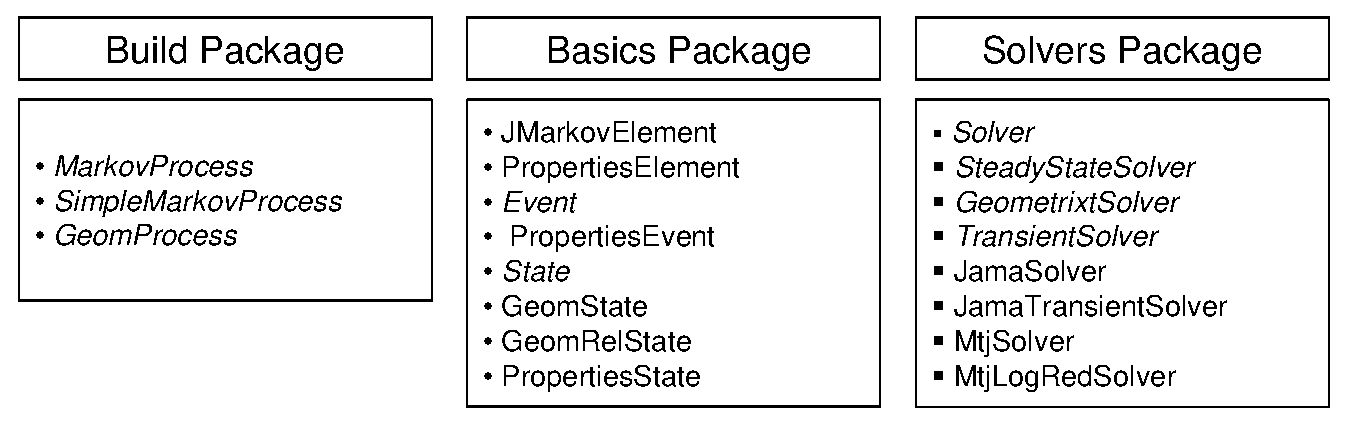
\includegraphics[width=12cm]{pics/classClassification}
  \caption{Class classification}\label{fg:classClassification}
\end{figure*}

\subsection{Build Package}\label{sc:BuildModule}

The build package is the main one in jMarkov since it contains
the classes that take care of building the state space and transition matrices. %
The main classes are \MarkovProcess, \SimpleMarkovProcess,
and \GeomProcess (see Figure \ref{fg:BuildModuleDiag}). %
Wher\-eas the first two allow to model general Markov processes, \GeomProcess is
used for Quasi-Birth and Death Processes (QBD) and its description
is given in Section \ref{sec:QBDmodule} below.

\begin{figure}[htb]
  % Requires \usepackage{graphicx}
  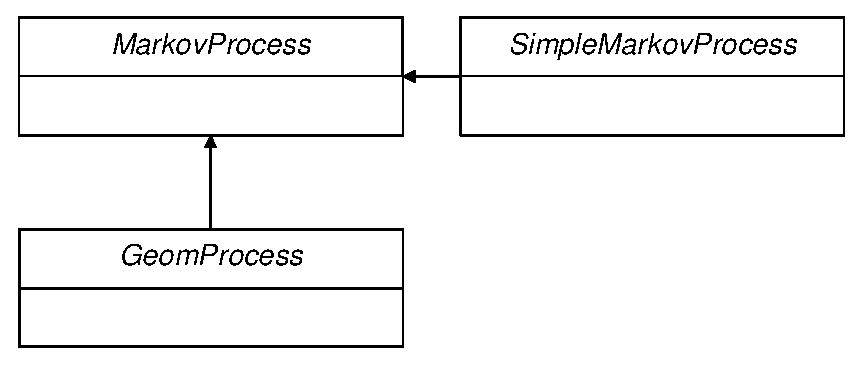
\includegraphics[width=0.95\columnwidth]{pics/buildModuleDiag}
  \caption{Class diagram build module}\label{fg:BuildModuleDiag}
\end{figure}

The class \SimpleMarkovProcess represents a Markov cha\-in process, and contains
three abstract methods that implement the three aforementioned functions
in the algorithm BuildRS: \Active, \Dests, and \Rate. %
In order to model a problem the user has to extend this class and
implement the three functions. %
An example is given in Section \ref{sec:Usage}. %
The class \MarkovProcess is the main class in the module, and
provides a more general mechanism to describe the dynamics of the
system. %
It also contains tools to communicate with the solvers to
compute steady state and transient solutions, and print them in a
diverse array of ways. %
For details, see \cite{rian.goez:jmarkovManual}.


\subsection{Basic Package}\label{sc:BasicModule}


This package contains the building blocks needed to describe a Markov Chain. %
It contains classes such as \texttt{State}, and \texttt{Event}, which allow
the user to code a description of the states and events, respectively
(see Figure \ref{fg:basicModuleDiag}). %
The user has freedom to choose any particular coding that best
describes the states in her model, like any combination of integers, strings, etc. %
However, she must establish a complete ordering among the elements since,
for efficiency, jMarkov works with ordered sets. %
For simplicity, however, a built-in class is provided,
called \texttt{PropertiesState}, that describes the state with
an array of integers, something which is quite appropriate for many applications. %
Similarly, there is an analogous class called \texttt{PropertiesEvent}. %
The package also contains the classes \texttt{States} and \texttt{Events}
that are used to describe collections of states and events. %
These are fairly general classes, since all that is required from
the user is to provide a mechanism to ``walk through'' the elements of
the set, taking advantage of Java iterator mechanism. %
This implies that, for large sets, there is no need to
generate (and store) all the elements in the set. %
For convenience, the package provides  implementations of these
set classes based on sorted sets classes available in Java.


\begin{figure}[htb]
    \centering
  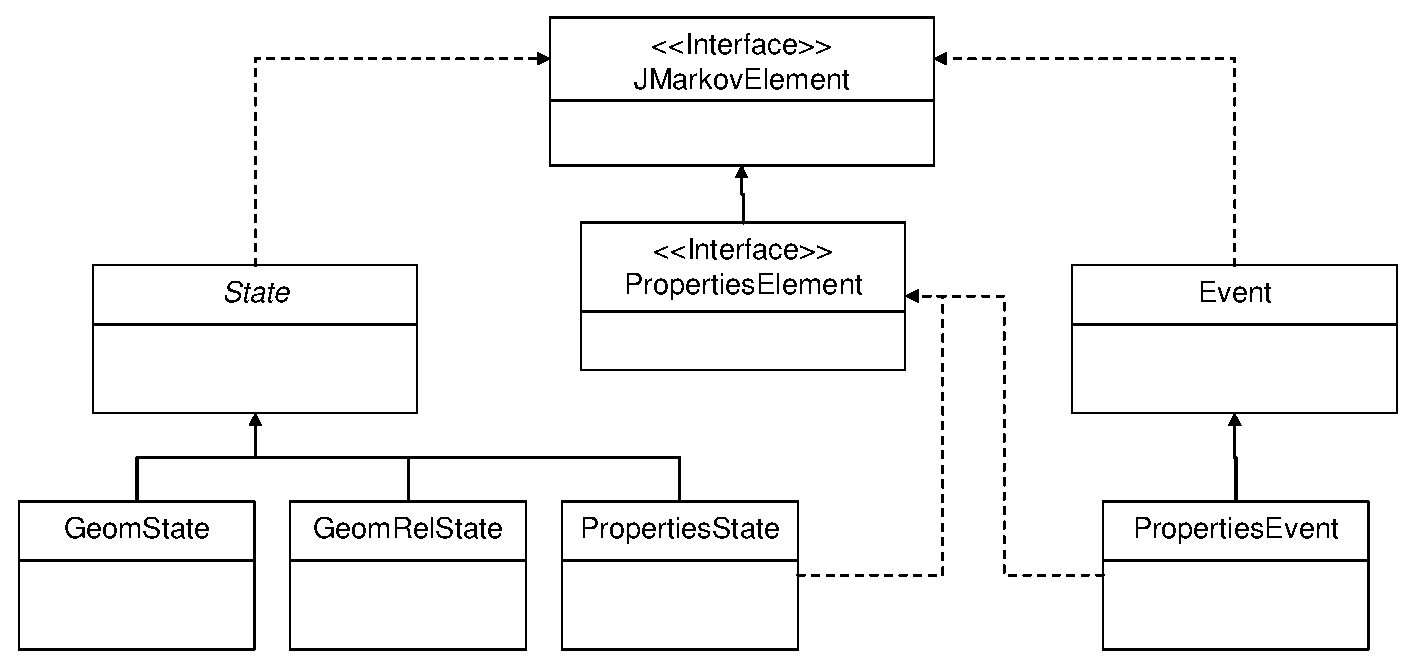
\includegraphics[width=0.95\columnwidth]{pics/basicModuleDiag}
  \caption{Class diagram for the basic package}\label{fg:basicModuleDiag}
\end{figure}


\subsection{The Solvers Package}\label{sec:SolversModule}

As stated above, jMarkov separates modeling from solving. %
Various solvers are provided to find steady-state and
transient probabilities (see Figure \ref{fg:SolversModuleDiag}). %
If the user does not specify the solver to use, one is provided by default. %
However, the architecture is flexible enough to allow an interested
user to choose a different solver, or, if she desires, to implement her own. %
The basic class is called \texttt{Solver}, that has two sub-classes
called \texttt{Steady\-State\-Solver}, \texttt{Transient\-Solver},
and \texttt{Geom\-Solver} (see Figure \ref{fg:SolversModuleDiag}). %
As the names indicate, the first two provide solvers for steady
state and transient probabilities, whereas the latter is used
for QBDs, as explained in section \ref{sec:QBD}. %
The implementations provided relay on two popular Java packages to
handle matrix operations JAMA~\cite{hick.clev.ea05} and MTJ~\cite{Heim05}, for
dense and sparse matrices, respectively.



\begin{figure}[htb]
    \centering
  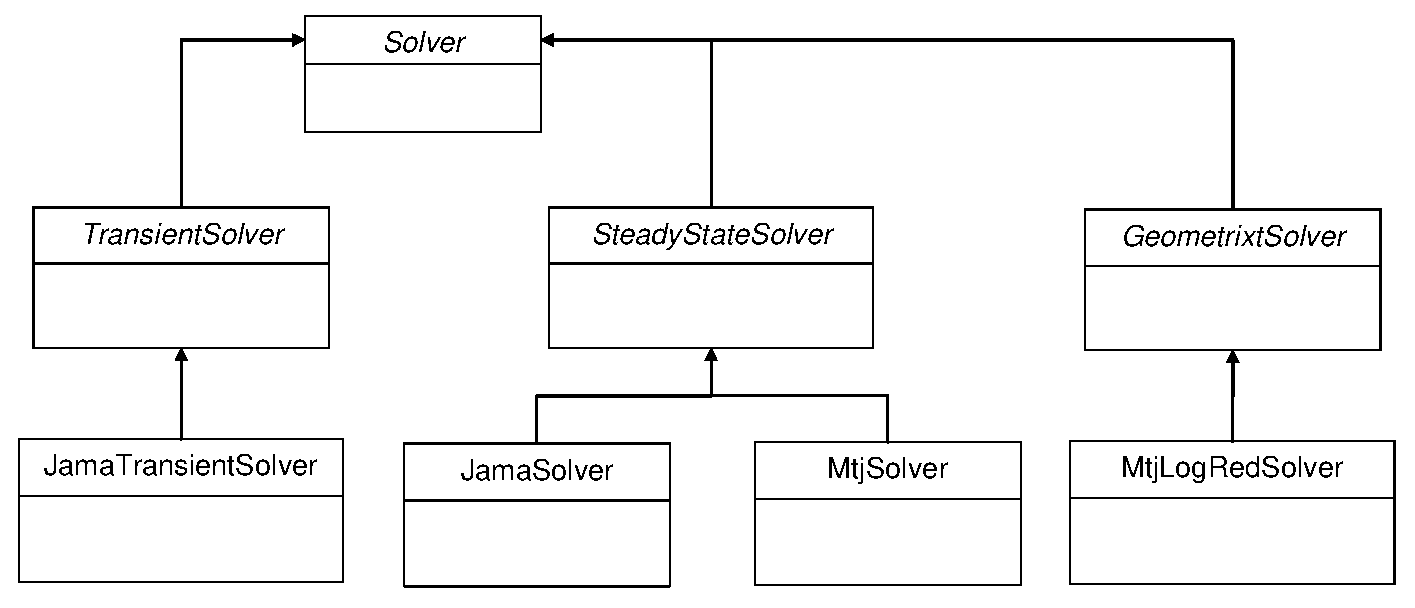
\includegraphics[width=0.95\columnwidth]{pics/SolversModuleDiag}
  \caption{Class diagram of the solvers package}\label{fg:SolversModuleDiag}
\end{figure}



\section{Examples}

\subsection{Example: An  M/M/2/N with different servers}

Assume that a system has Poisson arrivals with rate $\lambda$.
There are two exponential servers with rates $\mu_1$ and $\mu_2$
respectively. There is a maximum of $N$ customers in the system.
An arriving customer that finds the system empty will go to server
1 with probability $\alpha$. Otherwise he will pick he first
available server, or join a single FCFS queue. If there are $N$ in
the system the customer goes away.

\subsubsection{The model}
\newcommand{\bX}{\ensuremath{\mathbf X}}
We model this system with the triple $\bX(t) = (X(t),Y(t),Z(t))$,
where $X(t)$ and $Y(t)$ represents the status of the server (1 if
busy 0 otherwise) and $Z(t)$ represents the number in queue, which
is a number from 0 to $N-2$. There are $2 \times 2\times N-2$
potential states, however not all combinations of $X,Y$ and $Z$
are possible. For example the state $(0,1,2)$ is not acceptable
since we assume that a server will not be idle if there are people
in the queue. The set of states will be of the form
\[\cS=\{(0,0,0),(0,1,0),(1,0,0)\} \cup \{(1,1,k): k=
0,1,\ldots,N-2\}\]

The transition matrix will have the form


% Table generated by LaTeXcel from sheet 'Sheet1'
\begin{tabular}{r|r|r|r|r|r|r|r|r|r|}

                &             000 &             010 &             100 &             110 &             111 &             112 &        $\ldots$ &         1,1,N-3 &         1,1,N-2 \\
\cline{2-10}
            000 &                 & $\lambda\alpha$ & $\lambda(1-\alpha)$ &                 &                 &                 &                 &                 &                 \\
\cline{2-10}
            010 &         $\mu_2$ &                 &                 &       $\lambda$ &                 &                 &                 &                 &                 \\
\cline{2-10}
            100 &         $\mu_1$ &                 &                 &       $\lambda$ &                 &                 &                 &                 &                 \\
\cline{2-10}
            110 &                 &         $\mu_1$ &         $\mu_2$ &                 &       $\lambda$ &                 &                 &                 &                 \\
\cline{2-10}
            111 &                 &                 &                 &                 &                 &       $\lambda$ &                 &                 &                 \\
\cline{2-10}
            112 &                 &                 &                 &                 &   $\mu_1+\mu_2$ &                 &                 &                 &                 \\
\cline{2-10}
       $\vdots$ &                 &                 &                 &                 &                 &                 &                 &                 &                 \\
\cline{2-10}
        1,1,N-3 &                 &                 &                 &                 &                 &                 &                 &                 &       $\lambda$ \\
\cline{2-10}
        1,1,N-2 &                 &                 &                 &                 &                 &                 &                 &   $\mu_1+\mu_2$ &                 \\
\cline{2-10}
\end{tabular}





\subsubsection{Class QueueMM2dNState}
Our characterization of each state  fits nicely as a particular
case of the PropertiesState class with three properties. Since we
decided to work with numbered events rather than extending the
Event class, we should implement the \verb"SimpleMarkovClass". In
the following code you will see how we first model the State with
the class \verb"QueueMM2dNState" and then model the system
implementing the class \verb"QueueMM2dN". These two class are
placed in the same file QueueMM2dN, but they could be placed in
separate files.

To model the State we begin by creating a constructor that assigns
x, y, and z to the properties. We provide methods to access the
three properties and a method to check whether the system is
empty. We also implement the method label to override the one in the class PropertiesState.

\subsubsection{Class QueueMM2dN}


There are two basic events that can occur: arrivals and service
completions. We have to distinguish, however two types of service
completions depending on whether the server that finishes is 1 or
2. Also, when the system is empty we have to distinguish between
arrivals that go to server 1 and those that go to server 2. So in
total we have five events which we number as follows


\subsubsection{Code}
\lstinclude{QueueMM2dN.java}

\subsection{Multiple Server Queue}
In this example we generalize what we did in the previous example.
Assume that a system has exponential arrivals with exponential
arrivals. There are $K$ distinct servers with service rates
$\mu_1, \mu_2, \ldots, \mu_K$. A customer that finds all servers
busy joins a single FCFS queue, with capacity $N-K$ (so there will
be at most $N$ customers in the system). A customer that finds all
servers idle will choose among the idle servers according to
relative intensities $\alpha_k$, i.e., he will choose server $k$
with probability
\[\beta_k = \frac{\alpha_k}{\sum_{\ell\in \cal I}\alpha_{\ell}}, \qquad k \in \cal I\]
where $\cal I$ is the set of available servers.

\subsubsection{The model}

For this model we characterize each state by $X(t)=(S(t), Q(t))$,
where $S(t)=(S_1(t), \ldots, S_K(t))$, where $S_k(t)= 1$ if $k$-th
server is busy and 0 otherwise. The events that can occur are
arrivals and departures. However we  have to distinguish two type
of arrivals. If there is no idle server the arriving customer
joins the queue, and we will call this a non-directed arrival.
Otherwise we call it a directed arrival. We also make part of the
event description the server where the arrival is directed. In
order to represent this event we need a more sophisticated
structure, so instead of just numbering the events we rather
extend the class Event, creating an object with two integer fields
(components): the type and the server. Then it is very easy to
implement the functions \texttt{active, dest} and \texttt{rate}
just by querying the values of the type and server associated with
the state.

\subsubsection{Code}
\lstinclude{QueueMMKdN.java}


\subsection{Drive Thru}
\subsubsection{Code}
\lstinclude{DriveThru.java}

\subsubsection{Results}

\begin{lstlisting}[title={Output for Drive Thru}]
SISTEMA DRIVE THRU.
Tasa de Entrada   = 80.0
Tasa en el Mic    = 120.0
Tasa de sevicio 2 = 30.0
Posici{\'o}n del mic  = 5
Servidores        = 4
Cap en el sistema = 14



System has 498 States.


MEASURES OF PERFORMANCE

NAME                                       MEAN      SDEV
Tamano Cola                               4.503     2.693
Serv Ocupados Microfono                   0.550     0.498
Serv Ocupados Cocinando                   2.199     1.165
Serv Ocupados                             2.749     1.088
Clientes Bloqueados antes de ordenar      0.112     0.316
Clientes Bloqueados con orden lista       1.540     1.646
Clientes Bloqueados                       1.652     1.604
Total clientes en Espera                  6.155     3.487
Total Clientes                            8.903     3.396

EVENTS OCCURANCE RATES
NAME       MEAN RATE
Arrival       65.965
MicEnd        65.965
SrvEnd(0)     28.019
SrvEnd(1)      9.927
SrvEnd(2)      9.446
SrvEnd(3)      8.333
SrvEnd(4)      6.114
SrvEnd(5)      4.126

Tiempo de espera para Tamano Cola: 4.096 minutos
Tiempo de espera para Serv Ocupados Microfono : 0.5 minutos
Tiempo de espera para Serv Ocupados Cocinando: 2 minutos
Tiempo de espera para Serv Ocupados : 2.5 minutos
Tiempo de espera para Clientes Bloqueados antes de ordenar: 0.102 minutos
Tiempo de espera para Clientes Bloqueados con orden lista: 1.4 minutos
Tiempo de espera para Clientes Bloqueados: 1.503 minutos
Tiempo de espera para Total clientes en Espera: 5.598 minutos
Tiempo de espera para Total Clientes : 8.098 minutos
\end{lstlisting}

\section{Modeling Quasi-Birth and Death Processes}\label{sec:QBD}

In this section we give a brief description of Quasi-Birth and Death Processes (QBD), and explain how they can be modeled using jMarkov. QBD are Markov Processes with an infinite space state, but with a very specific repetitive structure that makes them quite tractable.

\subsection{Quasi-Birth and Death Processes}
\label{sec:QuasiBirthAndDeathProcesses}


Consider a Markov process $\{X(t):t\geq0\}$ with a two dimensional state space $\cS=\{(n,i):n \geq 0, 0\leq i\leq m \}$. The first coordinate $n$ is called the \emph{level} of the process and the second coordinate $i$ is called the \emph{phase}. We assume that the number of phases $m$ is finite. In applications, the level usually represents the number of items in the system, whereas the phase might represent different stages of a service process.

We will assume that, in one step transition, this process can go only to the states in the same level or to adjacent levels. This characteristic is analogous to a Birth and Death Process, where the only allowed transitions are to the two adjacent states (see, e.g \cite{kulk95}). Transitions can be from state $(n,i)$ to state $(n',i')$ only if $n' = n$, $n'=n-1$ or $n'=n+1$, and, for $n\ge 1$ the transition rate is independent of the level $n$. Therefore, the generator matrix, $\bQ$, has the following structure
\begin{equation*}\label{eq:QBDMatrix}
\bQ=
        \begin{bmatrix}
          \bB_{00}& \bB_{01}&             &             &  \\
          \bB_{10}& \bA_1& \bA_0&             &  \\
                        & \bA_2& \bA_1& \bA_0&  \\
                        &             & \ddots      & \ddots      & \ddots
        \end{bmatrix},
\end{equation*}
where, as usual, the rows add up to 0. An infinite Markov Process with the conditions described above is called a Quasi-Birth and Death Process (QBD).


In general, the level zero might have  a number of phases $m_0\neq m$. We will call these first $m_0$ states the \textit{boundary states}, and all other states will be called \textit{typical states}. Note that matrix $\bB_{00}$ has size $m_0\times m_0$, whereas $\bB_{01}$ and $\bB_{10}$ are matrices of sizes $(m_0\times m)$ and $(m \times m_0)$, respectively. Assume that the QBD is an ergodic Markov Chain. As a result, there is a steady state distribution $\bpi$ that is the
unique solution $\bpi$ to the system $\bpi \bQ = \zero$,
$\bpi \one = 1$.
Divide this $\bpi$ vector by levels, analogously to the way $\bQ$ was divided, as
\[ \bpi = [ \bpi_0, \bpi_1,\ldots]. \]
Then, it can be shown that a solution exist that satisfy
\[  \bpi_{n+1}= \bpi_n\bR, \qquad n > 1,\]
where $\bR$ is a constant square matrix of order $m$ \cite{neut81}.
This $\bR$ is the solution to the equation
\[ \bA_0 + \bR\bA_1  + \bR^2\bA_2  = \zero. \]
There are various algorithms that can be used to compute the matrix $\bR$. For example, you can start with any initial guess $\bR_0$ and obtain a series of $\bR_k$ through iterations of the form
\[ \bR_{k+1} = -(\bA_0 + \bR^2_k\bA_2 )\bA_1^{-1}. \]
This process is shown to converge (and $\bA_1$ does have an
inverse). More elaborated algorithms are presented in  Latouche
and Ramaswami \cite{lato.rama99}. Once $\bR$ has been determined
then $\bpi_0$ and $\bpi_1$ are determined by solving the following
linear system of equations
\begin{gather*}
        \begin{bmatrix}
            \bpi_0 & \bpi_1
        \end{bmatrix}
        \begin{bmatrix}
        \bB_{00} & \bB_{01}\\
        \bB_{10} & \bA_1 + \bR\bA_2\\
        \end{bmatrix}
         =
        \begin{bmatrix}
            \zero  & \zero
        \end{bmatrix}
\\
         \bpi_0 \one + \bpi_1(\bI-\bR)^{-1}\one = 1.
\end{gather*}

\subsection{Measures of performance for QBDs}
We consider two types of measures of performance that can be defined in a QBD model. The first type can be seen as a reward $r_i$ received whenever the system is in phase $i$, independent of the level, for level $n\ge1$. The long-run value for such a measure of performance is computed according to
\[ \sum_{n=1}^\infty \bpi_n \br = \bpi_1(\bI-\bR)^{-1}\br, \]
where $\br$ is an $m$-size column vector with components $r_i$. The second type of reward has the form $nr_i$, whenever the system is in phase $i$ of level $n$. Its long-run value is
\[\sum_{n=1}^\infty n \bpi_n \br = \bpi_1\bR(\bI-\bR)^{-2}\br. \]
%%%%%%%%%%%%%%%%%%%%%%%%%%%%%%%%%%%%%%%%%%%%%%%%
% This is used to equalize last page's columns:
\addtolength{\textheight}{-0cm}
%%%%%%%%%%%%%%%%%%%%%%%%%%%%%%%%%%%%%%%%%%%%%%%%


\subsection{Modeling QBD with jQBD}\label{sec:QBDmodule}

Modeling QBD with jMarkov is similar to modeling a Markov Processes. Again, the user has to code the states, the events, and then define the dynamics of the system through \Active, \Dests, and \Rate. The main difference is that special care needs to be taken when defining the destination states for the typical states. Rather than defining a new level for the destination state, the user should give a new \textit{relative} level, which can be -1, 0, or +1. This is accomplished by using two different classes to define states. The current state of the system is a \texttt{GeomState}, but the destination states are \texttt{GeomRelState}. The process itself must extend the class \GeomProcess, which in turn is an extension of \MarkovProcess.

The building algorithm uses the information stored about the dynamics of the process to explore the graph and build only the first three levels of the system. From this, it is straightforward to extract matrices $\bB_{00}$, $\bB_{01}$, $\bB_{10}$,  $\bA_0$, $\bA_1$, and $\bA_2$. Once these matrices are obtained,  the stability condition is checked. If the system is found to be stable, then the matrices $\bA_0$, $\bA_1$, and $\bA_2$ are passed to the solver, which takes care of computing the matrix $\bR$ and the steady state probabilities vectors $\bpi_0$ and $\bpi_1$, using the formulas described above. The implemented solver (\texttt{MtjLogRedSolver}) uses the logarithmic reduction algorithm \cite{lato.rama99}. This class uses MTJ for matrices manipulations.
There are also mechanisms to define both types of measures of performance mentioned above, and jQBD can compute the long run average value for all of them.


\subsection{An Example} \label{sec:Usage}

To illustrate the modeling process with jQBD,
we will show the previous steps with a simple example. %
Consider a infinite queue with a station that has a single
hiper-expo\-nen\-tial server with $n$ service phases, with
probability $\alpha_i$ to reach the service phase $i$ and
with service rate $\mu_i$ at phase $i$, where $0\leq i \leq n$. %
The station is fed from an external source according to a Poisson
processes with rate $\lambda$. %
We will use this model as an illustrative example of a QBD
process, and will show how each of the previous steps is performed
for this example. Of course all measures of performnce for this system can be readilly obtained in closed form since it is a particular case of an $M/G/1$, but we chose this example bacause of its simplicity. The code below actually models any general phase-type distribution, so the hyper-geometric will be a particular case.
\begin{itemize}
    \item \textbf{States:} Because of the memoryless property,
    the state of the system is fully characterized by an
    integer valued vector $\bx=(x_1, x_2)$, where $x_1 \geq 0$
    represents the number of items in the system and $0 \leq x_2 \leq n$
    represents the current phase of the service process.%
    Note that, knowing this, we can know how many 
    items are in service and how many are queuing. %
    It is important to highlight that the computational representation uses only the 
    phase of the system ($x_2$) because the level ($x_1$)is manged internally by the framework. %
    \item \textbf{Events:} An event occurs whenever an
    item arrives to the system or finishes processing at
    a particular service phase $0 \leq i \leq n$. %
    Therefore, we will define the set of possible events as
    $\cE =\{a, c_1, c_2, \ldots, c_n\} $, where the event $a$ 
    represents an arrival to the system and an event $c_i$ represents
    the completion of a service in phase $i$. 

\item   \textbf{Markov Process:} We elected to implement
\GeomProcess, which implied coding the following three methods:
\begin{itemize}
    \item \Active\texttt{(i,e)}: Since the queue is an infinite QBD
    process the event $a$ is always active, and the events
    $c_i, 0 \leq i \leq n$ are active
    if there is an item at workstation on service phase $i$. %
    The code to achieve this can be seen in Figure
    \ref{ls:HiperExQueueActiveMethod}. %
    \item \Dests\texttt{(i,e,j)}: When the event $a$ occurs there is always an
    increment on the system level, but you need to consider if the server is idle or busy. %
    When the server is idle the new costumer could start in any of the 
    $n$ service phases, then the system could reach anyone of the first level
    $n$ states with probability $\alpha_i$. On the other hand, if the server is 
    busy on service phase $i$, the system will reach the next level state with 
    the same service phase $i$. %
    
    On the other hand, when the server finishes one service $c_i$, no matter which phase type,
    the level of the system is reduced by one, but you need to consider if the system
    is in level 1 or if it is in level 2 or above. When the level is 1, the system 
    reach the unique state ($0,0$) where there are no costumer in the system and the server is idle.
    On the other hand, if the system level is equal or greater than 2, the system 
    could reach any of the $n$ states in the level below with probability $\alpha_i$.
    The Java code can be seen in Figure
    \ref{ls:HiperExQueueDestsMethod}. %
    \item \Rate\texttt{(i,e)}: The rate of occurrence of
    event $a$ is given simply by $\lambda$ and the rate of occurrence
    of an event $c_i$ is given by $\mu_i$. %
    In Figure \ref{ls:HiperExQueueRateMethod} you can see the corresponding
    code.
\end{itemize}
 \item \textbf{MOPs:} Using the MOPS types defined in jQBD component, we will
 illustrate its use calculating the expected WIP on the system.
\end{itemize}


%\begin{figure}[htb]
%  \centering
%  \lstinputlisting[linerange ={8-11}]{HiperExQueueState.java}
%  \caption{Constructor of class HiperExQueueState.java}
%  \label{ls:HiperExQueueStateConstructor}
%\end{figure}

%\begin{figure}[htb]
%  \centering
%  \lstinputlisting[linerange ={8-25}]{HiperExQueueEvent.java}
%  \caption{Constructor of class HiperExQueueEvent.java}
%  \label{ls:HiperExQueueEventConstructor}
%\end{figure}

\begin{figure}[htb]
  \centering
%  \lstinputlisting[linerange ={226-238}]{HiperExQueue.java}
  \lstinclude[linerange ={226-238}]{HiperExQueue.java}
  \caption{\texttt{Active} method of class HiperExQueue.java}
  \label{ls:HiperExQueueActiveMethod}
\end{figure}

\begin{figure}[htb]
  \centering
  \lstinclude[linerange ={245-273}]{HiperExQueue.java}
  \caption{\texttt{dests} method of class HiperExQueue.java}
  \label{ls:HiperExQueueDestsMethod}
\end{figure}

\begin{figure}[htb]
  \centering
  \lstinclude[linerange ={286-315}]{HiperExQueue.java}
  \caption{\texttt{rate} method of class
  HiperExQueue.java}
  \label{ls:HiperExQueueRateMethod}
\end{figure}





Finally, the output obtained after running the model can
be seen in the Graphical User Interface (GUI) in
Figure \ref{fg:GUIExample}. %
There is no need to use the GUI, but it is helpful
to do so during the first stages of development, to
make sure that all transitions are being generated as expected. %
All the measures of performance defined can be extracted
by convenience methods defined in the API or a report
printed to standard output. %
Such a report can be seen in  Figure \ref{fg:MOPs}.


\begin{figure*}[bt]
  % Requires \usepackage{graphicx}
  \centering
  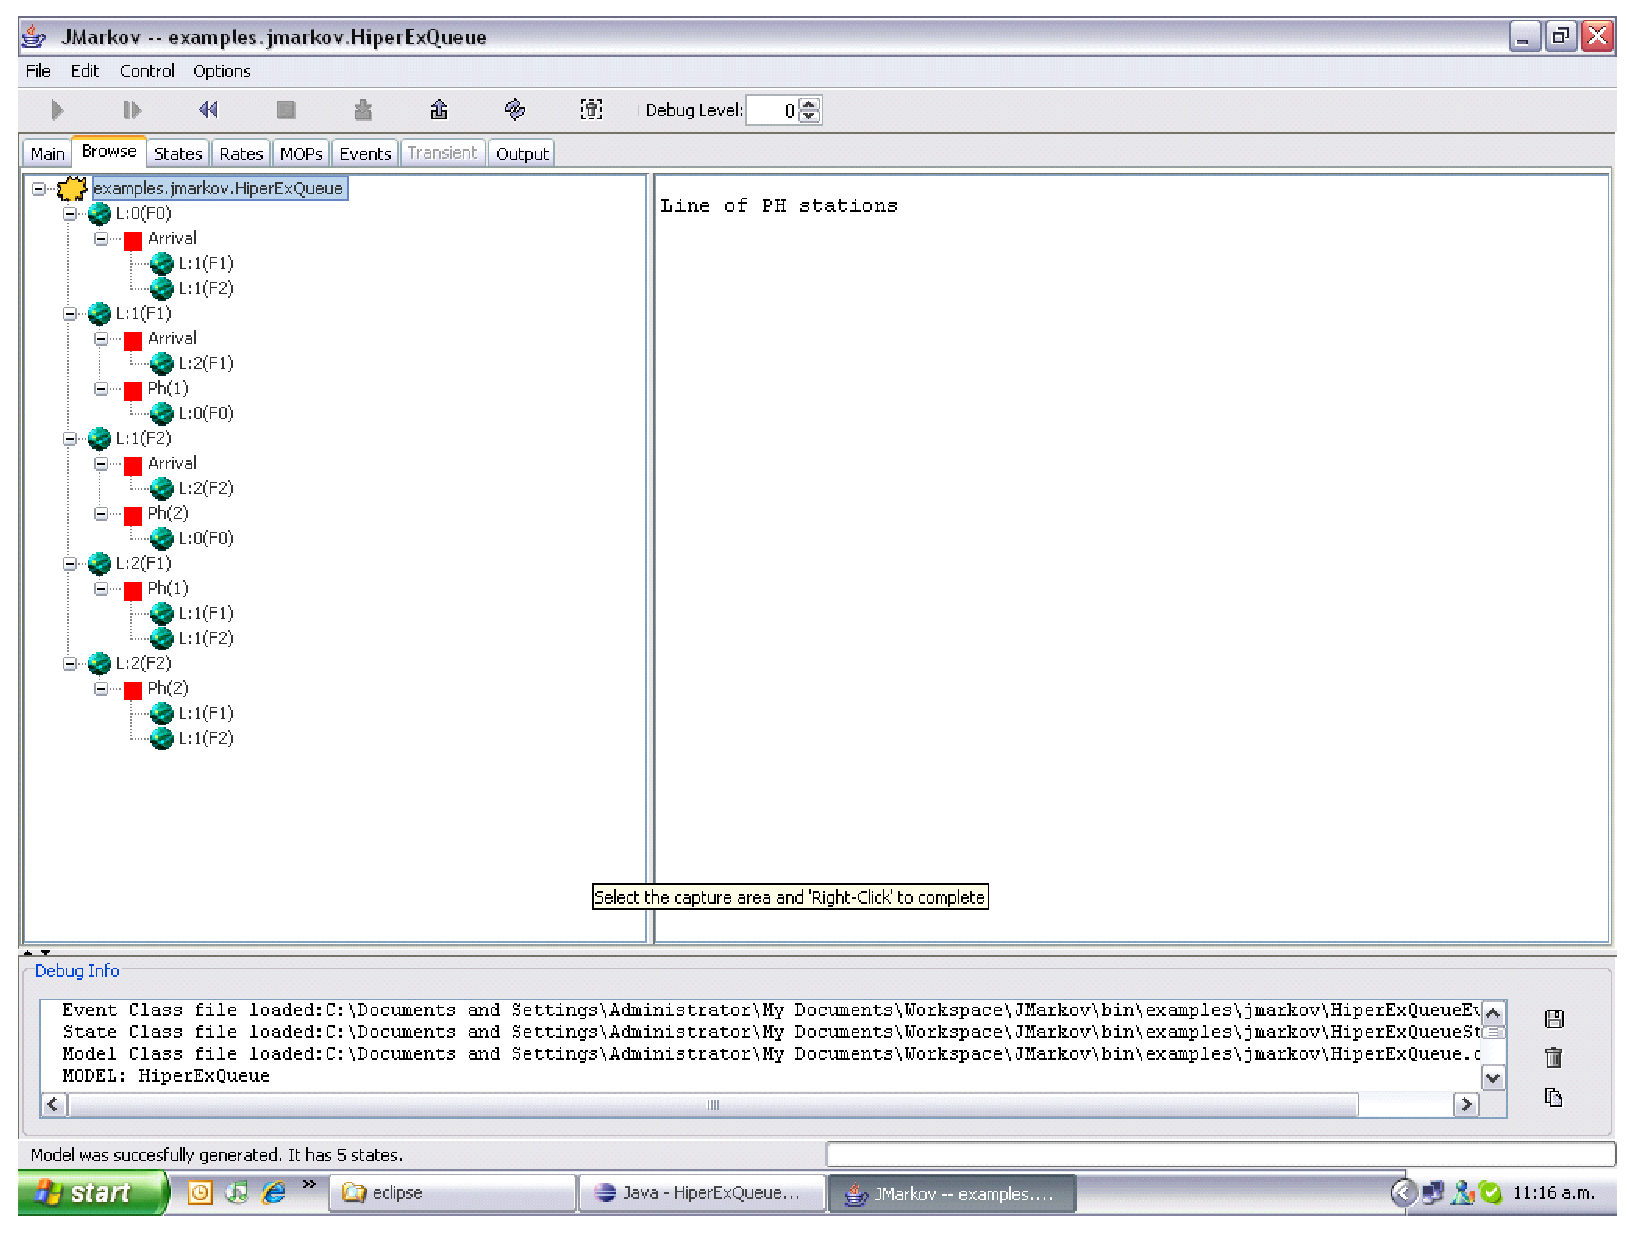
\includegraphics[width=0.9\textwidth,clip]{pics/GUIexampleQBD}
  \caption{GUI example of jMarkov}\label{fg:GUIExample}
\end{figure*}

\begin{figure}[htb]
\small
\begin{lstlisting}
MEASURES OF PERFORMANCE

NAME                     MEAN      SDEV

Expected Level        0.14286         ?
Server Utilization    0.12500   0.33072

\end{lstlisting}
\caption{MOPs report of jMarkov}\label{fg:MOPs}
\end{figure}

\section{Advanced Features}

\subsection{Using the Solvers}




\subsection{Using the Transitions scheme}



\subsection{Computing MOPs on the fly to save memory}


\subsection{extending jMarkov}



\section{Further Development}

This project is currently under development, and therefore we appreciate all the feedback we can receive.

\bibliographystyle{abbrv}
\addcontentsline{toc}{section}{References}
\bibliography{%
../../Papers/Biblio/ComputerScience,%
../../Papers/Biblio/Stochastics,%
../../Papers/Biblio/Optimization,%
../../Papers/Biblio/Riano,%
../../Papers/Biblio/Manufacturing,%
../../Papers/Biblio/Math%
}


%\begin{thebibliography}{Dillo 83}
%\bibitem{bellman} Bellman, Richard. \emph{Dynamic Programming}. Princeton, New Jersey: Princeton University Press, 1957.
%
%\bibitem{bertsekas} Bertsekas, Dimitri. \emph{Dynamic Programming and Optimal Control} Belmont, Massachusetts: Athena Scientific, 1995.
%
%\bibitem{bjorn} Bjorn-Ove, Heinsund. \emph{JMP-Sparce Matrix Library in Java}, Department of Mathematics, University of Bergen, Norway, September 2003.
%
%\bibitem{ciardo}Ciardo, Gianfranco. \textit{Tools for Formulating Markov Models} in ``Computational Probability'' edited by Winfried Grassman. Kluwer Academic Publishers, USA, 2000.
%
%\bibitem{mp:mdp} Puterman, Martin. \textit{Markov Decision Processes}. John Wiley \& Sons Inc.
%
%\bibitem{stidham} Stidham, J. \emph{Optimal Control of Markov Chains} in ``Computational Probability'' edited by Winfried Grassman. Kluwer Academic Publishers, USA, 2000.
%
%\bibitem{ld:jj} Van der Linden, Peter. \textit{Just Java}. The sunsoft
%Press. 1996
%
%\end{thebibliography}



\printindex


\end{document}
